% #############################################################################
% This is Chapter 4
% !TEX root = ../main.tex
% #############################################################################
% Change the Name of the Chapter i the following line
\fancychapter{Dataset Construction}
\cleardoublepage
% The following line allows to ref this chapter
\label{chap:implement}

This chapter presents the systematic approach for constructing the AerialD dataset for open-vocabulary aerial image segmentation. Our methodology transforms existing aerial datasets into a comprehensive referring segmentation resource through automated rule-based generation and LLM enhancement.

% #############################################################################
\section{Source Datasets}

\noindent The AerialD dataset is constructed from two primary sources of aerial imagery with fundamentally different annotation paradigms, as illustrated in Table~\ref{tab:dataset_sources}. The iSAID dataset is an instance segmentation dataset providing high-resolution aerial images with precise boundaries for individual object instances across fifteen categories including ships, vehicles, planes, buildings, and infrastructure elements such as harbors and bridges. In contrast, the LoveDA dataset is a semantic segmentation dataset that captures land cover and land use patterns, providing pixel-level classification into categories such as buildings, water bodies, agricultural areas, forests, and barren land. These two datasets ensure comprehensive coverage of both discrete objects and continuous landscape features commonly encountered in aerial imagery analysis.


% Dataset sources table with images
\begin{table}[H]
\centering
\caption{Source Dataset Characteristics}
\label{tab:dataset_sources}
\begin{tabular}{@{}p{4cm}p{8cm}@{}}
\toprule
\multicolumn{2}{c}{\textbf{iSAID Dataset}} \\
\midrule
\raisebox{-0.5\height}{\includegraphics[width=3.5cm, height=3.5cm]{./Images/isaid.png}} & 
\hspace{-0.5cm}\parbox[c]{8cm}{\fontsize{10pt}{12pt}\selectfont Contains \textbf{2,806} high resolution images at varying widths of 800 to 13,000 pixels, spatial resolution of \textbf{0.1m to 4.5m}, with \textbf{655,451} instances across \textbf{15} object classes including \textbf{ships}, \textbf{large vehicles}, \textbf{small vehicles}, \textbf{planes}, etc.} \\[0.5cm]
\midrule
\multicolumn{2}{c}{\textbf{LoveDA Dataset}} \\
\midrule
\raisebox{-0.5\height}{\includegraphics[width=3.5cm, height=3.5cm]{./Images/loveda_dataset.png}} & 
\hspace{-0.5cm}\parbox[c]{8cm}{\fontsize{10pt}{12pt}\selectfont Contains \textbf{5,987} images at 1024 pixel width, spatial resolution of \textbf{0.3m}, across \textbf{6} land cover classes: \textbf{building}, \textbf{road}, \textbf{water}, \textbf{barren}, \textbf{forest}, and \textbf{agriculture}.} \\[0.5cm]
\bottomrule
\end{tabular}
\end{table}

% #############################################################################
% #############################################################################
\section{Rule-Based Expression Generation}

The rule-based expression generation pipeline systematically transforms semantic segmentation and instance segmentation datasets into referring expression datasets through a sequential five-step process that analyzes spatial, visual, and relational properties of objects and groups within aerial imagery. This comprehensive approach begins with patch extraction from source datasets and culminates in linguistically diverse and contextually accurate referring expressions.

The process initiates with iSAID patch extraction, where instance annotations are loaded from COCO-format JSON files containing 655,451 instances across 15 object categories. The system extracts 480$\times$480 patches using a sliding window approach with 20\% overlap, processing both training and validation splits through multiprocessing for computational efficiency. The sliding window approach creates the risk that objects may be partially cut off at patch boundaries, where a cutoff object is defined as an instance whose segmentation polygon extends beyond the extracted patch area. Critical to maintaining annotation quality, the extraction process handles cutoff objects by calculating intersection ratios, marking instances where less than 50\% remains within patch boundaries and fewer than 500 pixels are visible as potentially unreliable. Polygon segmentations are converted to run-length encoding (RLE) format for storage efficiency, while we extract essential metadata from JSON annotations including bounding boxes, areas, and segmentation data. The system filters out patches with excessive black pixels exceeding a 50\% threshold, ensuring visual content quality throughout the dataset.

LoveDA patch processing follows a distinct approach tailored to semantic segmentation data from 1024$\times$1024 images across urban and rural domains. The system resizes the entire image to 480$\times$480 dimensions to maintain consistency with iSAID patches. For ``building'' and ``water'' categories, the system converts semantic segmentation masks into individual instance segmentation masks through connected components analysis. This selective conversion makes sense because LoveDA's land cover classification design means that buildings and water bodies naturally occur as discrete, spatially bounded entities with clear geometric boundaries, making them suitable for instance segmentation. In contrast, classes such as agriculture, forest, and barren land represent diffuse land cover types that extend across large continuous regions without natural instance boundaries, making individual instance extraction neither meaningful nor reliable for these categories.

For LoveDA building and water categories, individual instances are extracted using connected components analysis, which identifies spatially connected regions within each semantic class by examining pixel connectivity patterns. The algorithm traverses the binary mask where pixels are considered connected if they are adjacent horizontally, vertically, or diagonally, meaning each pixel can connect to any of its eight neighboring pixels in the surrounding 3$\times$3 grid, effectively grouping contiguous pixels belonging to the same semantic class into distinct labeled regions. Connected components below minimum area thresholds of 50 pixels for buildings and 100 pixels for water are filtered out to eliminate spurious detections. This dual-layer processing creates both individual building and water instances for referring expression generation, while simultaneously preserving the complete semantic segmentation masks containing all pixels of each class. Agricultural areas, forests, and barren land are exclusively treated as unified semantic classes, with single masks encompassing all pixels of each category and pre-written expressions such as ``all buildings in the image'' generated for these class-level groups, while multiprocessing handles both urban and rural domains efficiently.

The core rule addition and analysis phase transforms basic annotations into rich spatial and visual descriptions through systematic feature extraction. Each 480$\times$480 patch undergoes partitioning into a three-by-three grid establishing nine distinct spatial regions, with sophisticated borderline detection using an alpha parameter of 0.2 to create neutral zones for ambiguous boundary cases. Color classification operates on HSV pixels extracted from segmentation masks, distinguishing achromatic colors (light and dark) using a saturation threshold below 25\% and chromatic colors across eight hue ranges including red, orange, yellow, green, cyan, blue, purple, and magenta. Dominance thresholds of 70\% for both achromatic and chromatic classifications ensure reliable color assignment, while ambiguous cases maintain multiple possible color alternatives. Extreme position detection identifies topmost, bottommost, leftmost, and rightmost instances within each category using margin-based separation criteria, while size relationship analysis determines largest and smallest objects through area-based comparisons with threshold ratios.

Spatial relationship calculation employs an angle-based directional system spanning eight compass directions, with distance-based filtering using dynamic thresholds adjusted according to object sizes to include only meaningful nearby relationships. The system handles borderline relationships by recording multiple directional possibilities when objects fall near angular boundaries. Group formation utilizes DBSCAN clustering with parameters eps=40, minimum samples of 2, and maximum samples of 8, operating separately within each object category to maintain semantic coherence. Class-level groups are automatically generated for categories containing multiple instances, creating expressions like ``all ships in the image'', while special pair groups combine small and large vehicles when both types coexist within patches.

\begin{figure}[H]
\centering
\begin{minipage}{0.5\textwidth}
\centering
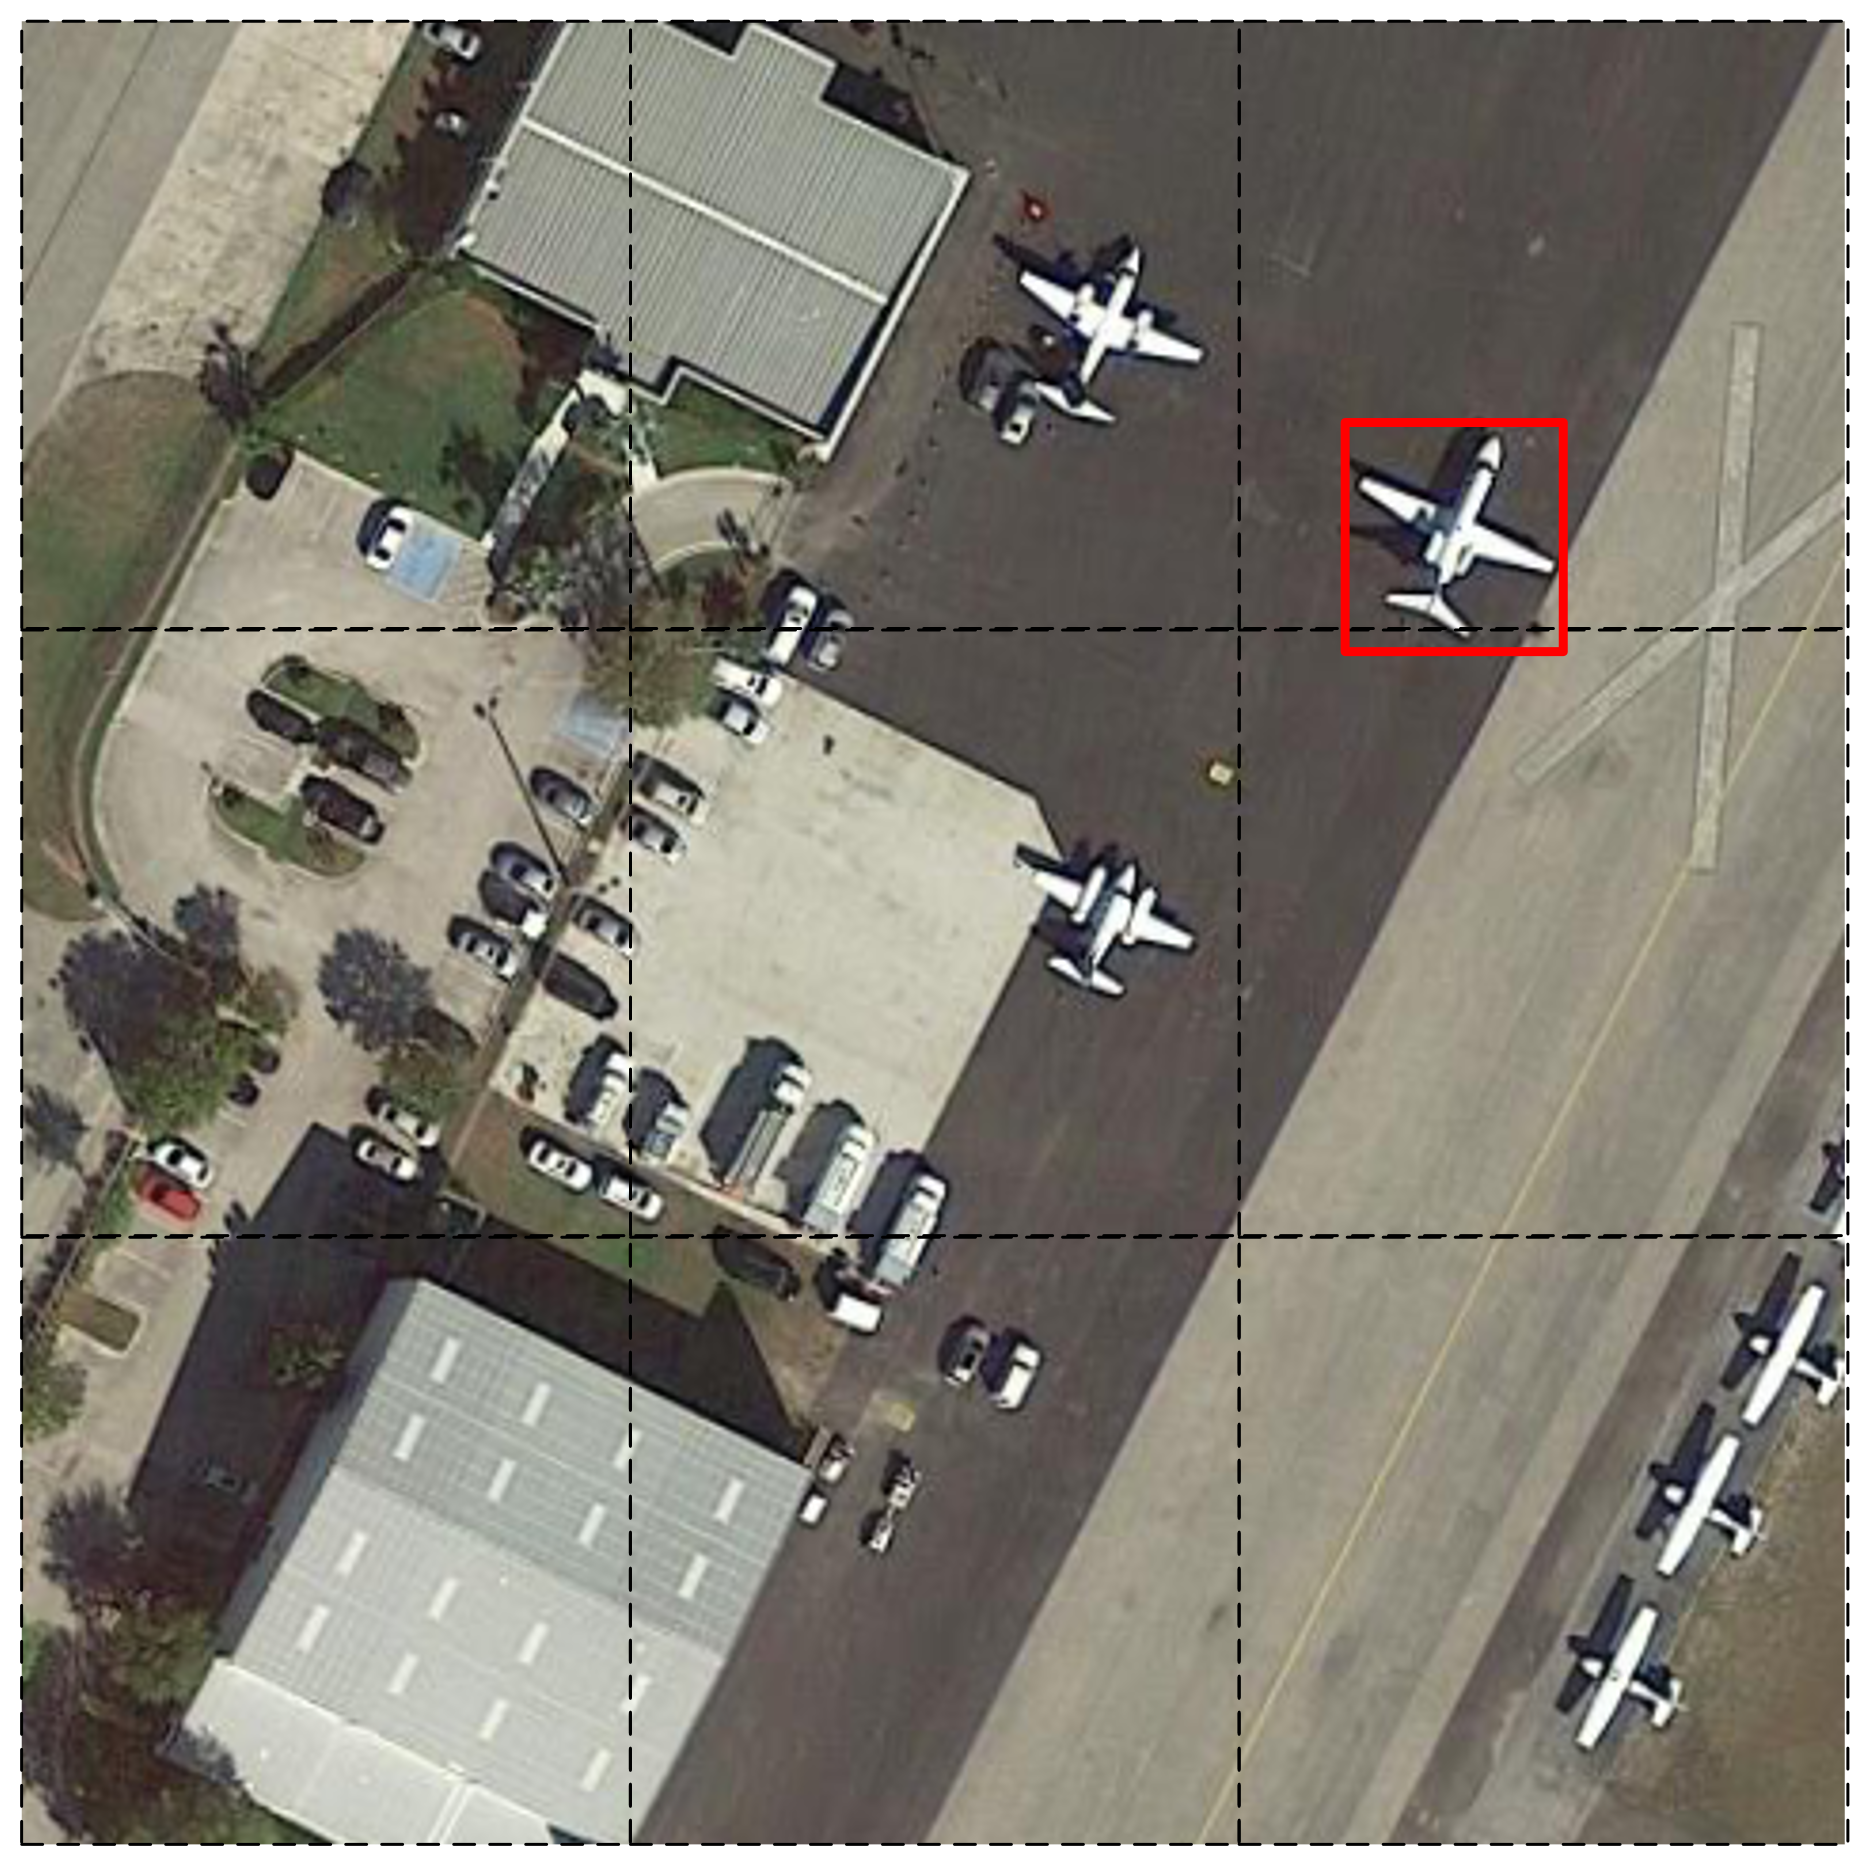
\includegraphics[width=0.7\textwidth]{./Images/rule_based_generation.png}
\end{minipage}%
\begin{minipage}{0.5\textwidth}
\centering
\hspace{-1cm}
\raisebox{-0.3\height}{%
\resizebox{\textwidth}{!}{%
\footnotesize
\begin{tabular}{@{}ll@{}}
\toprule
\textbf{Rule Type} & \textbf{Example Instance} \\
\midrule
Category & "plane" \\
Grid Position & "in the top right" \\
Extreme Position & None \\
Color Classification & "light" \\
Directional Relations & "to the bottom right of a plane" \\
& "to the top right of a plane" \\
\midrule
\multicolumn{2}{l}{\textbf{Final Expressions}} \\
\multicolumn{2}{l}{"the plane in the top right"} \\
\multicolumn{2}{l}{"the light plane in the top right"} \\
\multicolumn{2}{l}{"the plane in the top right to the bottom right of a plane"} \\
\multicolumn{2}{l}{"the light plane in the top right to the bottom right of a plane"} \\
\multicolumn{2}{l}{"the plane in the top right to the top right of a plane"} \\
\multicolumn{2}{l}{"the light plane in the top right to the top right of a plane"} \\
\bottomrule
\end{tabular}%
}%
}
\end{minipage}
\caption{Example of rule generation for a single instance. The highlighted plane in the top right section demonstrates how the system assigns spatial, visual, and relational rules that will later be combined into referring expressions.}
\label{fig:rule_example}
\end{figure}

The expression generation engine operates through combinatorial synthesis of extracted attributes, creating comprehensive linguistic descriptions by systematically enumerating all valid combinations of category labels, grid positions, spatial relationships, extreme positions, size characteristics, and color properties. The system implements seventeen distinct expression templates ranging from simple category-only descriptions like ``the ship'' to complex multi-attribute formulations such as ``the dark largest ship in the top right that is above a building''. Color expression filtering removes chromatic color references from buildings and water to maintain semantic appropriateness, while borderline cases generate multiple expression variants to ensure comprehensive coverage of spatial and relational interpretations. Group expressions handle multi-instance clusters with appropriate size quantifiers and plural forms, while dummy expression marking tags potentially unreliable expressions originating from cutoff objects or ambiguous relationships for subsequent filtering.

Uniqueness filtering ensures expression quality and eliminates ambiguity through systematic standardization and deduplication processes. The system converts class names from technical formats to natural language equivalents, transforming ``Large\_Vehicle'' to ``large vehicle'' and applying appropriate pluralization logic based on group sizes and context. Expression standardization normalizes linguistic variations while preserving semantic meaning, followed by duplicate detection that identifies and removes expressions appearing multiple times across the dataset. The strict deduplication policy eliminates all occurrences of non-unique phrases, preventing ambiguous references that would compromise the referring expression task. Dummy expressions from cutoff objects are removed after uniqueness checking to maintain only high-confidence annotations, while objects and groups lacking valid expressions are eliminated entirely from the dataset.

% Expression uniqueness filter example
\begin{figure}[H]
\centering
\begin{minipage}{0.5\textwidth}
\centering
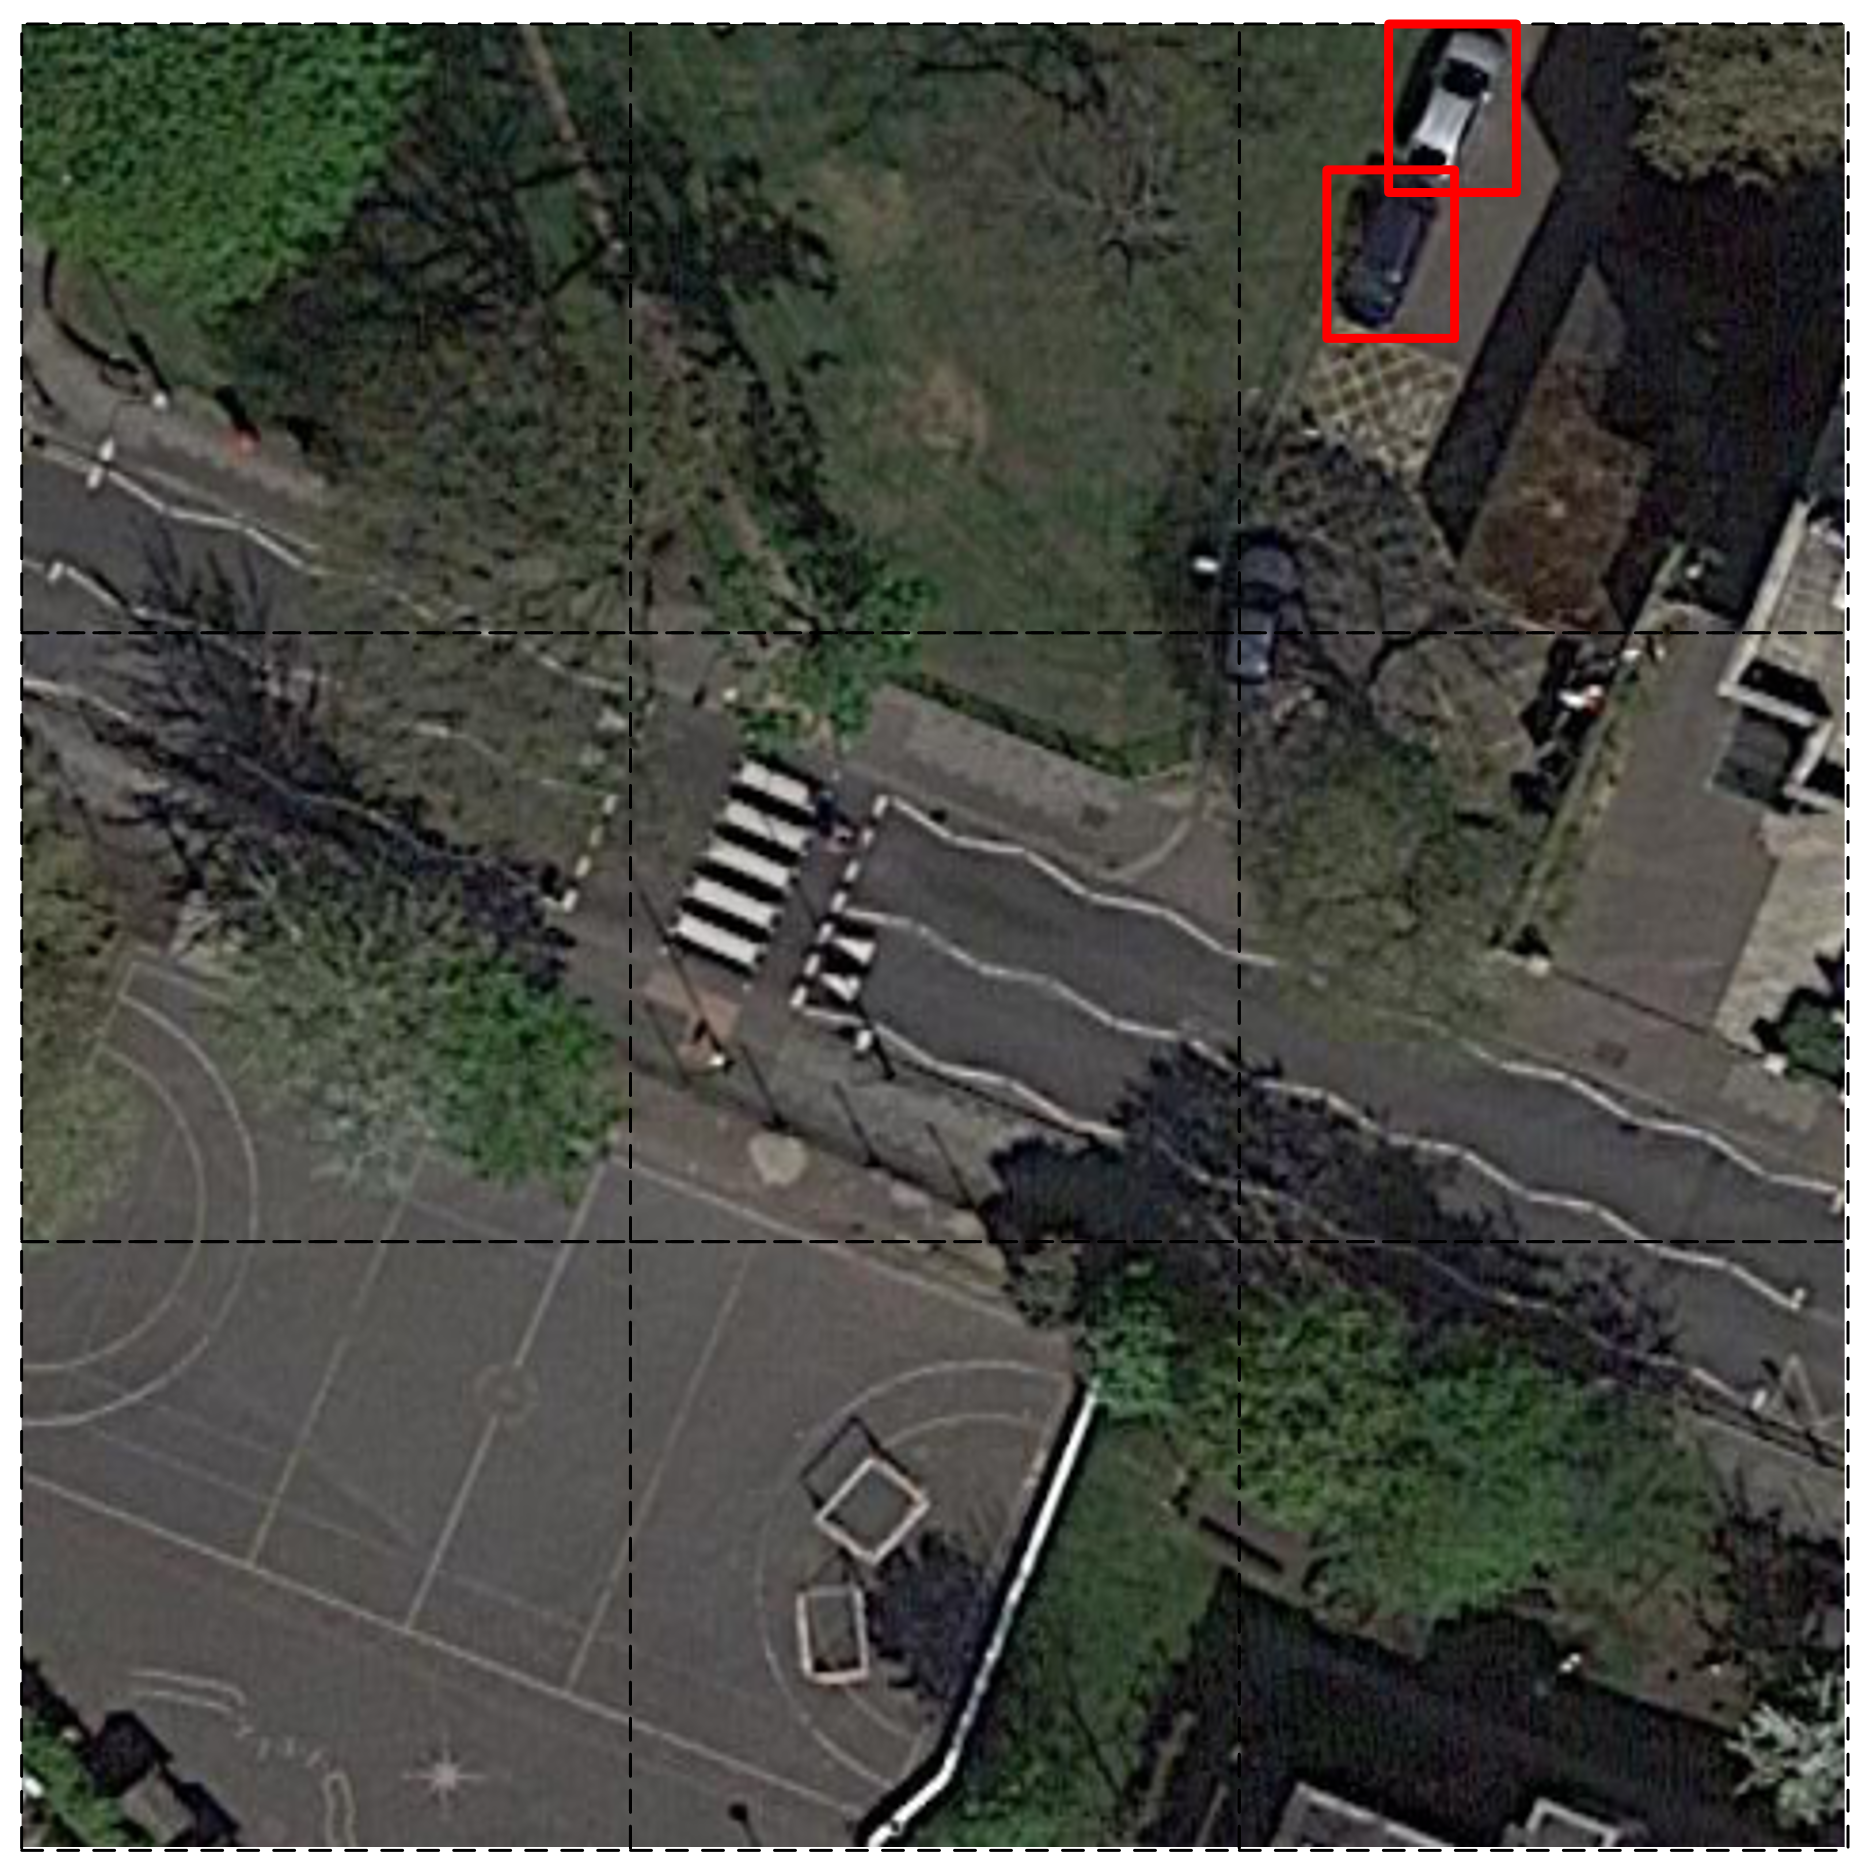
\includegraphics[width=0.7\textwidth]{./Images/filter_unique.png}
\end{minipage}%
\begin{minipage}{0.5\textwidth}
\centering
\hspace{-1cm}
\raisebox{-0.3\height}{%
\resizebox{\textwidth}{!}{%
\footnotesize
\begin{tabular}{@{}ll@{}}
\toprule
\textbf{Expression} & \textbf{Status} \\
\midrule
\multicolumn{2}{l}{\textbf{Object 1 (Light Vehicle)}} \\
\midrule
"the small vehicle in the top right" & \textcolor{red}{Filtered} \\
"the topmost small vehicle" & \textcolor{green!70!black}{Kept} \\
"the light small vehicle in the top right" & \textcolor{green!70!black}{Kept} \\
"the light topmost small vehicle" & \textcolor{green!70!black}{Kept} \\
"the small vehicle in the top right above a small vehicle" & \textcolor{green!70!black}{Kept} \\
\midrule
\multicolumn{2}{l}{\textbf{Object 2 (Dark Vehicle)}} \\
\midrule
"the small vehicle in the top right" & \textcolor{red}{Filtered} \\
"the dark small vehicle in the top right" & \textcolor{green!70!black}{Kept} \\
"the small vehicle in the top right below a small vehicle" & \textcolor{green!70!black}{Kept} \\
\bottomrule
\end{tabular}%
}%
}
\end{minipage}
\caption{Example of expression uniqueness filtering showing how ambiguous expressions are removed when multiple objects occupy similar spatial positions. The blue and red boxes highlight two small vehicles in the top right corner that would create conflicting references.}
\label{fig:uniqueness_filter}
\end{figure}



% #############################################################################
\section{LLM Expression Generation}

Beyond rule-based expression generation, we further enhance the dataset through multimodal large language model fine-tuning. We leverage the generalization capabilities of open-source multimodal LLMs, which possess both advanced language understanding and vision processing capabilities, to create more natural and diverse referring expressions. Through fine-tuning a multimodal LLM specifically on the task of expression enhancement, we apply this enhanced model to the full extent of our rule-based dataset, more than doubling the number of expressions from the original rule-based generation and significantly increasing the linguistic diversity and naturalness of the referring expressions.

% LLM enhancement example figure
\begin{figure}[H]
\centering
\begin{minipage}{0.5\textwidth}
\centering
\includegraphics[width=0.7\textwidth]{./Images/example_group.png}
\end{minipage}%
\begin{minipage}{0.5\textwidth}
\centering
\hspace{-1cm}
\raisebox{-0.3\height}{%
\footnotesize
\begin{tabular}{@{}p{2cm}p{5cm}@{}}
\toprule
\textbf{Expression Type} & \textbf{Example} \\
\midrule
Original & the group of 4 large vehicles in the top center \\
\midrule
Enhanced & the cluster of four big vehicles near the upper middle \\
\midrule
Unique & the four large vehicles lined up side by side just below the pale paved strip at the very top middle \\
\midrule
Unique & the set of four big vehicles parked in a single row in the upper center beside the grassy area to the right \\
\bottomrule
\end{tabular}%
}
\end{minipage}
\caption{Example of LLM enhancement process showing original aerial image with group of four large vehicles (left) and corresponding expression enhancements (right).}
\label{fig:llm_enhancement_example}
\end{figure}

% #############################################################################
\section{LLM Distillation}

Knowledge distillation enables scalable enhancement of the full dataset by transferring capabilities from large proprietary models to smaller, locally deployable models.

\begin{figure}[H]
\centering
\includegraphics[width=0.8\textwidth]{./Images/distillation.png}
\caption{Knowledge distillation pipeline for scalable LLM enhancement. A small sample of 500 expressions is processed through OpenAI's O3 model to generate high-quality training targets, which are then used to fine-tune Gemma3 12B via QLora. The fine-tuned model enables cost-effective local inference to enhance the full dataset of 300,000 expressions using vLLM on a single GPU.}
\label{fig:llm_distillation}
\end{figure}


% #############################################################################
\section{Final Dataset Statistics}

The completed AerialD dataset represents a comprehensive resource for aerial referring expression segmentation, combining rule-based generation with LLM enhancement to create diverse and natural language descriptions.

% Dataset examples figure
\begin{figure}[H]
\centering
\includegraphics[width=\textwidth]{./Images/dataset.png}
\caption{Representative examples from AerialD dataset showing diverse referring expressions with corresponding aerial images and ground truth masks.}
\label{fig:dataset_examples}
\end{figure}

% Dataset statistics table
\begin{table}[H]
\centering
\caption{Dataset Statistics Summary}
\label{tab:dataset_stats}
\begin{tabular}{@{}lrrr@{}}
\toprule
\textbf{Metric} & \textbf{Train} & \textbf{Val} & \textbf{Total} \\
\midrule
Total Patches & 27,480 & 9,808 & 37,288 \\
Individual Objects with Expressions & 94,179 & 34,536 & 128,715 \\
Individual Expressions & 646,686 & 242,668 & 889,354 \\
Groups with Expressions & 96,832 & 34,162 & 130,994 \\
Group Expressions & 471,108 & 162,061 & 633,169 \\
Total Samples & 191,011 & 68,698 & 259,709 \\
Avg. Expressions per Individual Object & 6.87 & 7.03 & 6.91 \\
Avg. Expressions per Group & 4.87 & 4.74 & 4.83 \\
\bottomrule
\end{tabular}
\end{table}

% Category distribution table
\begin{table}[H]
\centering
\caption{Object Category Distribution by Instance Type and Source Dataset}
\label{tab:category_dist}
\resizebox{\textwidth}{!}{%
\begin{tabular}{@{}lrrrrr@{}}
\toprule
\textbf{Category} & \textbf{Individual Instances} & \textbf{Groups} & \textbf{Instance Expressions} & \textbf{Group Expressions} & \textbf{Source Dataset} \\
\midrule
Ship & 11,461 & 10,402 & 79,251 & 49,272 & iSAID \\
Large Vehicle & 17,425 & 18,496 & 121,593 & 95,356 & iSAID \\
Small Vehicle & 41,353 & 53,682 & 262,831 & 282,848 & iSAID \\
Storage Tank & 2,985 & 3,451 & 19,537 & 16,071 & iSAID \\
Harbor & 9,164 & 6,290 & 72,248 & 28,613 & iSAID \\
Swimming Pool & 3,147 & 1,999 & 23,355 & 10,011 & iSAID \\
Tennis Court & 3,492 & 2,364 & 25,116 & 9,959 & iSAID \\
Soccer Ball Field & 1,781 & 569 & 13,939 & 2,368 & iSAID \\
Roundabout & 924 & 278 & 6,452 & 1,220 & iSAID \\
Basketball Court & 959 & 636 & 7,339 & 2,757 & iSAID \\
Bridge & 3,300 & 1,267 & 23,085 & 5,269 & iSAID \\
Ground Track Field & 1,368 & 208 & 9,111 & 868 & iSAID \\
Plane & 10,774 & 7,260 & 78,808 & 32,057 & iSAID \\
Helicopter & 354 & 266 & 2,636 & 1,144 & iSAID \\
Baseball Diamond & 1,049 & 381 & 7,965 & 1,576 & iSAID \\
Vehicle Pair & 0 & 7,597 & 0 & 30,388 & iSAID \\
Building & 10,341 & 3,012 & 66,038 & 12,048 & LoveDA \\
Water & 8,838 & 2,917 & 70,050 & 11,668 & LoveDA \\
Road & 0 & 3,018 & 0 & 12,072 & LoveDA \\
Agriculture & 0 & 2,342 & 0 & 9,368 & LoveDA \\
Barren & 0 & 1,709 & 0 & 6,836 & LoveDA \\
Forest & 0 & 2,850 & 0 & 11,400 & LoveDA \\
\bottomrule
\end{tabular}%
}
\end{table}

% Expression taxonomy table with counts
\begin{table}[H]
\centering
\caption{Complete Taxonomy of Generated Expression Types}
\label{tab:expression_types}
\resizebox{\textwidth}{!}{%
\begin{tabular}{@{}cccccrl@{}}
\toprule
\textbf{Category} & \textbf{Position} & \textbf{Extreme} & \textbf{Color} & \textbf{Relationship} & \textbf{Total Count} & \textbf{Example} \\
\midrule
\multicolumn{7}{l}{\textbf{Individual Instance Expressions}} \\
\midrule
\checkmark & & & & & 5,157 & "the ship" \\
\checkmark & \checkmark & & & & 26,437 & "the ship in the bottom right" \\
\checkmark & \checkmark & & & \checkmark & 25,403 & "the ship in the bottom right that is to the left of a harbor" \\
\checkmark & & \checkmark & & & 22,930 & "the topmost ship" \\
\checkmark & \checkmark & \checkmark & & & 22,930 & "the topmost ship in the top left" \\
\checkmark & \checkmark & \checkmark & & \checkmark & 9,761 & "the topmost ship in the top left that is above a building" \\
\checkmark & & & \checkmark & & 19,172 & "the dark ship" \\
\checkmark & \checkmark & & \checkmark & & 58,252 & "the dark ship in the bottom right" \\
\checkmark & \checkmark & & \checkmark & \checkmark & 42,165 & "the dark ship in the bottom right that is to the left of a harbor" \\
\checkmark & & \checkmark & \checkmark & & 35,571 & "the dark topmost ship" \\
\checkmark & \checkmark & \checkmark & \checkmark & & 35,571 & "the dark topmost ship in the top left" \\
\checkmark & \checkmark & \checkmark & \checkmark & \checkmark & 15,242 & "the dark topmost ship in the top left that is above a building" \\
\midrule
\multicolumn{7}{l}{\textbf{Group Expressions}} \\
\midrule
\checkmark & \checkmark & & & & 40,281 & "the group of 3 ships in the center" \\
\checkmark & \checkmark & & & \checkmark & 86,307 & "the group of 3 ships in the center that is above a group of 2 buildings" \\
\checkmark & & & & & 61,015 & "all buildings in the image" \\
\bottomrule
\end{tabular}%
}
\end{table}

% LLM enhancement stats table
\begin{table}[H]
\centering
\caption{LLM Enhancement Expression Distribution}
\label{tab:llm_enhancement_stats}
\begin{tabular}{@{}lrrr@{}}
\toprule
\textbf{Expression Source} & \textbf{Train} & \textbf{Val} & \textbf{Total} \\
\midrule
Rule-Based Expressions & 371,360 & 134,834 & 506,194 \\
LLM Enhanced (Language Variations) & 364,396 & 132,499 & 496,895 \\
LLM Unique (Visual Details) & 382,038 & 137,396 & 519,434 \\
\midrule
\textbf{Total Expressions} & \textbf{1,117,794} & \textbf{404,729} & \textbf{1,522,523} \\
\bottomrule
\end{tabular}
\end{table}

The construction of the AerialD dataset represents a significant advancement in aerial referring expression segmentation resources, providing comprehensive coverage of object categories, spatial relationships, and linguistic diversity. The resulting dataset serves as a foundation for training and evaluating sophisticated referring segmentation models that can understand complex natural language descriptions in aerial imagery contexts.



